\documentclass[a4paper]{article}
\usepackage{url}
\usepackage[utf8]{inputenc}
\usepackage{fancyvrb}
\usepackage{hyperref}

\title{Posłowie na Sejm RP 7 kadencji wg stażu}
\author{Tomasz Przechlewski}
\usepackage{Sweave}
\begin{document}
\maketitle

Zbiór \url{sejm7_wg_stazu.csv} zawiera m.in. informacja o~liczbie kadencji
na jaką został wybrany poseł (kolumna \texttt{kadencje}). Wartość minimalna
w~tej kolumnie 
wynosi $1$ dla posła wybranego po raz pierwszy do Sejmu~7 kadencji.

\begin{Schunk}
\begin{Sinput}
> ## Pierszy wiersz pliku CSV: imnz;rokur;klub;kadencje
> poslowie <- read.csv("sejm7_wg_stazu.csv", sep = ';',  header=T);
\end{Sinput}
\end{Schunk}

\begin{figure}[!tbh]
\begin{Schunk}
\begin{Sinput}
> boxplot(kadencje~klub, poslowie )
\end{Sinput}
\end{Schunk}
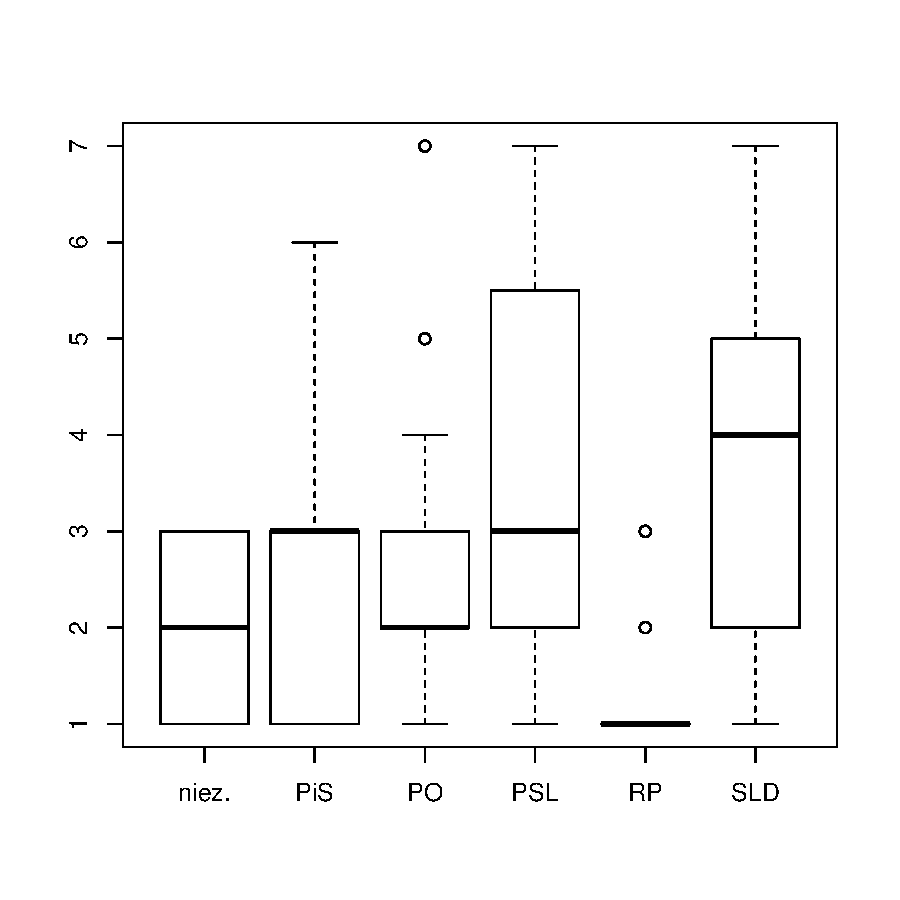
\includegraphics{sejm7_wg_stazu-002}
\caption{Średni staż posłów (wykres pudełkowy)}
\end{figure}

Średni staż posłów w~poszczegółnych klubach:

\begin{Schunk}
\begin{Sinput}
> tapply (poslowie$kadencje, poslowie$klub, mean)
\end{Sinput}
\begin{Soutput}
   niez.      PiS       PO      PSL       RP      SLD 
2.500000 2.737179 2.497585 3.642857 1.097561 3.615385 
\end{Soutput}
\end{Schunk}

Posłowie~7 kadencji Sejmu według klubów i~liczby kadencji:

\begin{Schunk}
\begin{Sinput}
> # http://ww2.coastal.edu/kingw/statistics/R-tutorials/descriptive.html
> table(poslowie$klub, poslowie$kadencje)
\end{Sinput}
\begin{Soutput}
         1  2  3  4  5  6  7
  niez.  1  0  0  1  0  0  0
  PiS   48 26  5 74  2  1  0
  PO    50 82  1 72  1  0  1
  PSL    5  5  4  5  2  4  3
  RP    39  1  0  1  0  0  0
  SLD    5  3  0 11  5  0  2
\end{Soutput}
\end{Schunk}

\end{document}
